\chapter{Experimental Results and Comparative Analysis}

\section{Experiment Specifications and Used Materials}

This section presents and discusses all the details related to the experiments 
carried out to investigate and evaluate the performance of the proposed approaches. 
In this project, simulation experiments were performed on Google Colab with K80 GPU 
and 12 GB memory and a 16 GB RAM, Intel Core i7-4610M CPU (3.00 GHz, 1600 MHz, 4 MB 
L3 Cache, 2 cores, 37W).
The proposed approach is designed with Tensorflow, Keras, Pytorch using Python.

\section{Evaluation Metrics}

To evaluate the performance of the proposed system, several performance metrics, 
namely, Accuracy, Recall (Sensitivity) and Precision, were calculated according to 
equations (\ref{eq:evalacc})-(\ref{eq:evalrec})-(\ref{eq:evalpre}), respectively. where, TP is the true positive values, FP is 
the false positive values, TN is the true negative values, FN is the false negative 
values, and N is the total number of observations. \\\\

\begin{equation} \label{eq:evalacc}
  \text{Accuracy} \ = \ (T P + T N) \ / \ (T P + F N + T N + F P)
\end{equation}
\begin{equation} \label{eq:evalrec}
  \text{Recall\ (Sensitivity)} \ = \ T P \ / \ (T P + F N)
\end{equation}
\begin{equation} \label{eq:evalpre}
  \text{Precision} \ = \ T P \ / \ (T P + F P)
\end{equation}
{\bf TP}, {\bf FP}, {\bf TN}, and {\bf FN} terms are defined as follows:
\begin{itemize}
  \item \textbf{True Positive (TP):} the image is X and is classified as a X.
  \item \textbf{False Positive (FP):} the image is Y and is classified as a X.
  \item \textbf{True Negative (TN):} the image is Y and is classified as Y.
  \item \textbf{False Negative (FN):} the image is X and is classified as Y.
\end{itemize}


\section{Results of The System}

\subsection{Dataset description}

PlantVillage dataset is used to perform plant disease detection and Plants 
Identification. This dataset consists of 38 classes of different plants with total of 54303 healthy and unhealthy leaf 
images. It is also openly available on the internet. Each class contains 
approximately 2000 images. For every plant's health as well as diseased images 
of leaves are available. Figure (\ref{fig:samplehealth}) shows samples of healthy and unhealthy apple leaf. Most of the images belong to Tomato and Apple plants. 
The description of classes used in the system from this dataset is given in the
table (\ref{tblr:dataset}). \\\\

\begin{figure}[H]
    \centering
    \begin{tabular}{cccc}
        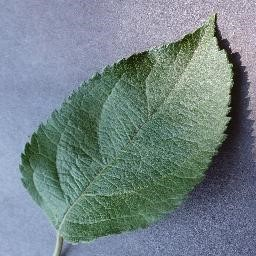
\includegraphics[width=3cm]{photos/chapter05/1.jpg} & 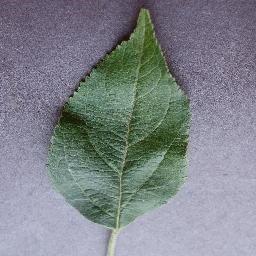
\includegraphics[width=3cm]{photos/chapter05/2.jpg} 
        & 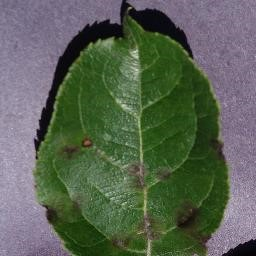
\includegraphics[width=3cm]{photos/chapter05/3.jpg} &  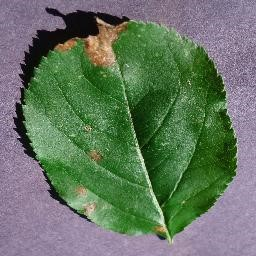
\includegraphics[width=3cm]{photos/chapter05/4.jpg} \\[3pt]
        \multicolumn{2}{c}{(a) Healthy} & \multicolumn{2}{c}{(b) Unhealthy} \\[1pt]
    \end{tabular}
    \caption{Samples of Healthy and Unhealthy Apple Leaf.}
    \label{fig:samplehealth}
\end{figure}

\begin{longtblr}[
  caption = {Datasets (PlantVillage) description.},
  label = {tblr:dataset},
] {
  colspec = {clclc}, width=\textwidth,
  rowhead = 2, rows={font=\fontsize{9}{9}},
  hlines, vlines,
  cell{1}{1} = {c=5}{c},
  cell{2}{1,2,3,4,5} = {c=1}{c},
  cell{27}{1} = {c=5}{c},
  cell{28}{1} = {c=3}{c},
  cell{28}{4} = {c=2}{c},
}

  \textbf{Dataset of plant disease detection and Plants Identification} \\
  \textbf{class} & \textbf{Plant Name} & \makecell{\textbf{Healthy} \\[-5pt] \textbf{or} \\[-5pt] \textbf{Diseased}} & \textbf{Disease Name} & \makecell{\textbf{Images}  \\[-3pt] \textbf{(Number)}} \\
  C\_0 & Apple & Diseased & Apple\_scab & 1,890 \\
  C\_1  & Apple &  Diseased & Black\_rot & 1,863 \\
  C\_2  & Apple & Diseased & Cedar\_apple\_rust & 825 \\
  C\_3  & Apple & Healthy & - & 4,935 \\
  C\_4  & Cherry\_(including\_sour) & Diseased & Powdery\_mildew & 3,156 \\
  C\_5  & Cherry\_(including\_sour) & Healthy & - & 2,562 \\
  C\_6  & Corn\_(maize) & Diseased & Cercospora\_leaf\_spotGray\_leaf\_spot & 1,539 \\
  C\_7  & Corn\_(maize) & Diseased & Common\_rust & 3,576 \\
  C\_8  & Corn\_(maize) & Diseased & Northern\_Leaf\_Blight & 2,955 \\
  C\_9  & Corn\_(maize) & Healthy & - & 3,486 \\
  C\_10  & Grape & Diseased & Black\_rot & 3,540 \\
  C\_11  & Grape & Diseased & Esca\_(Black\_Measles) & 4,149 \\
  C\_12  & Grape & Diseased & Leaf\_blight (Isariopsis\_Leaf\_Spot) & 3,228 \\
  C\_13  & Grape & Healthy & - & 1,269 \\
  C\_14  & Peach & Diseased & Bacterial\_spot & 6,891 \\
  C\_15  & Peach & Healthy & - & 1,080 \\
  C\_16 & Pepper\_bell & Diseased & Bacterial\_spot & 2,991 \\
  C\_17 & Pepper\_bell & Healthy & - & 4,434 \\
  C\_18 & Potato & Diseased & Early\_blight & 3,000 \\
  C\_19 & Potato & Diseased & Late\_blight & 3,000 \\
  C\_20 & Potato & Healthy & - & 456 \\
  C\_21 &Strawberry & Diseased & Leaf\_scorch & 3,327 \\
  C\_22 & Strawberry & Healthy & - & 1,368 \\
  C\_22 & Strawberry & Healthy & - & 1,368 \\

  \textbf{Dataset of ripeness assessment} \\
  Real Dataset of Strawberry & & & Number of images = 310 & \\
\end{longtblr}


\subsection{Results and Discussion}
The proposed approaches were implemented considering three scenarios:
\begin{itemize}
  \item Scenario I: Plants identification.
  \item Scenario II: Plant disease detection.
  \item Scenario III: Ripeness assessment.
\end{itemize}
Experimental results of the first two scenarios using both fine-tuned pre-trained 
Inception V3 and fine-tuned pre-trained VGG-16 models will be discussed in this 
section. The proposed Inception V3 model is trained using hyper-parameters 
(batch size = 64, epoch = 12). The VGG-16 model is trained using hyper-parameters 
(batch size = 32, epoch = 20). Experimental results of the third scenario using 
YOLOV5 model to recognize the ripeness stages in our dataset. The proposed YOLOV5 model is 
trained using hyper-parameters (batch size = 64, epoch = 150).


\subsubsection{Scenario I: Plants Identification}

This scenario presents plants identification model using raw data. 
The results of applying Inception V3 and VGG-16 fine-tuning procedures 
models on the PlantVillage dataset is discussed in this subsection. 
Table (\ref{tab:preform1}) shows the different performance metrics on dataset of 
the first scenario.

\begin{table}[H]
  \setlength\arrayrulewidth{0.5pt}
  \renewcommand{\arraystretch}{1.5}
  \begin{tabularx}{\textwidth}{|X|c|c|c|c|}
      \hline
      \multicolumn{5}{|c|}{\textbf{PlantVillage Dataset}} \\ \hline
      \textbf{Model} & \textbf{Accuracy} & \textbf{Recall} & \textbf{Precision} & \textbf{F - measure} \\ \hline
      \textbf{VGG-16 fine-tuning} & 98.2\% & 0.91 & 0.92 & 0.91 \\ \hline
      \textbf{Inception-V3}       & 100\%  & 0.99 & 0.99 & 0.99 \\ \hline
  \end{tabularx}
  \caption{Performance metrics for dataset of the Plants Identification model trained.}
  \label{tab:preform1}
\end{table}

Table (\ref{tab:preform1}) shows the performance of the Inception V3 and 
VGG-16 fine-tuning procedures models for classification considering PlantVillage
Dataset. For Inception V3 with PlantVillage Dataset, it is noticed that the obtained 
accuracy is 100\%. However, the obtained recall percentage is 99.00\%. 
On the other hand, for VGG-16 fine-tuning with PlantVillage Dataset, it 
is noticed that the obtained accuracy is 98.2\%. However, the obtained
recall percentage is 91.0\%, where the percentage of correctly recognized 
plant images against the total number of actual plant images has been increased 
and the performance is improved accordingly. It also noticed that the use of Inception 
V3 using PlantVillage Dataset increases the precision to 99.00\%. Accordingly, it is concluded
that the Inception V3 model in general improves the accuracy by 1.8\% and the F - measure by 8\% 
compared to the proposed VGG16 fine-tuning model on the dataset. 
Figure (\ref{fig:scenarioI}) shows Scenario I: Plant Confusion Matrix.
\begin{figure}[H]
  \centering
  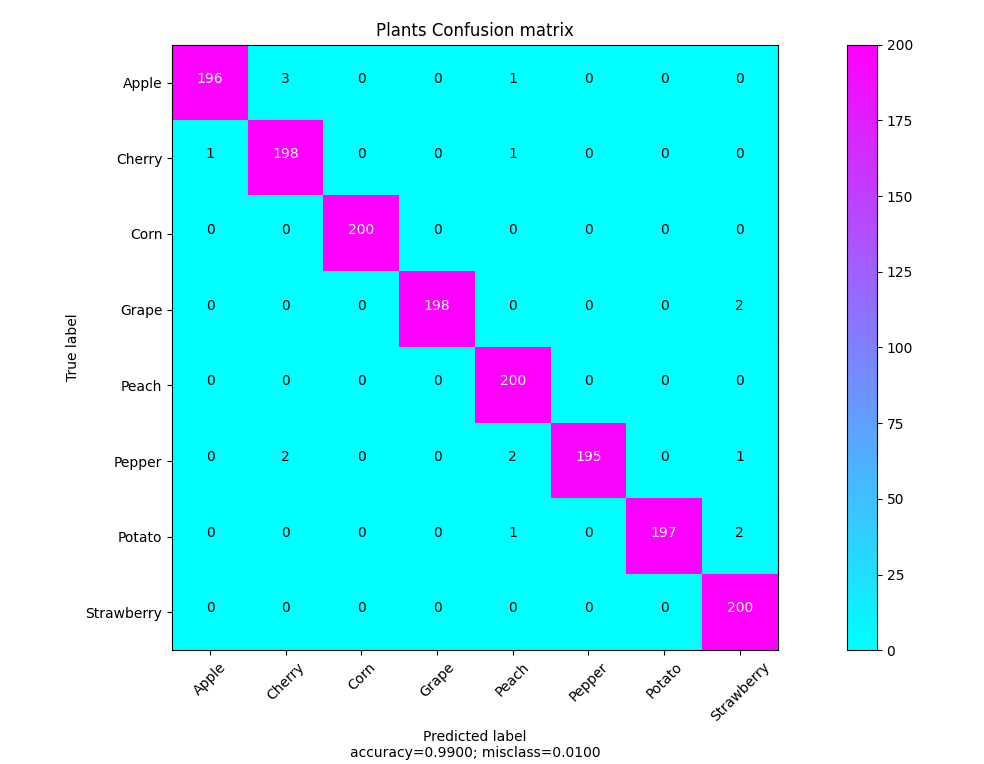
\includegraphics[width=12cm]{photos/chapter05/5.png}
  \caption{Scenario I: Plant Confusion Matrix.}
  \label{fig:scenarioI}
\end{figure}

\noindent Figure (\ref{fig:examplePlant}) shows Examples of Plants.
\begin{figure}[H]
  \centering
  \begin{tabular}{ccc}
      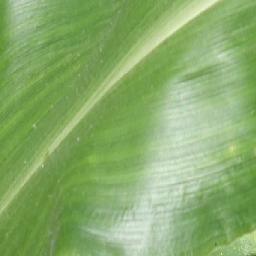
\includegraphics[width=4cm]{photos/chapter05/6.jpg} & 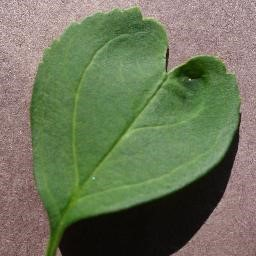
\includegraphics[width=4cm]{photos/chapter05/7.jpg} & 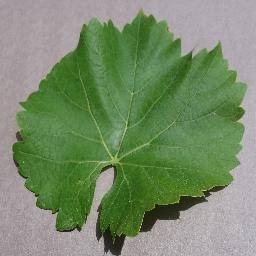
\includegraphics[width=4cm]{photos/chapter05/8.jpg} \\
  \end{tabular}
  \caption{Examples of Plants.}
  \label{fig:examplePlant}
\end{figure}

\subsubsection{Scenario II: Plant disease detection}

This scenario presents Plant disease detection Model using raw data. 
The results of applying Inception V3 on the PlantVillage dataset is discussed 
in this subsection. Table (\ref{tab:preform2}) shows the performance metrics of the eight models 
on dataset of the second scenario.

\begin{table}[H]
  \setlength\arrayrulewidth{0.5pt}
  \renewcommand{\arraystretch}{1.5}
  \begin{tabularx}{\textwidth}{|X|c|c|c|c|c|}
      \hline
      \multicolumn{6}{|c|}{\textbf{PlantVillage Dataset}} \\ \hline
      \multicolumn{1}{|c|}{\textbf{Model}} & \makecell{\textbf{Plant} \\[-4pt] \textbf{Name}} & \textbf{Accuracy} & \textbf{Recall} & \textbf{Precision} & \makecell{\textbf{F -} \\[-4pt] \textbf{measure}} \\ \hline
       & Strawberry & 100\%  & 1 & 1 & 1 \\ \cline{2-6}
       & Potato & 100\%  & 0.990 & 0.990 & 0.990 \\ \cline{2-6}
       & Pepper & 100\%  & 0.995 & 0.995 & 0.995 \\ \cline{2-6}
       & Peach & 100\%  & 0.995 & 0.995 & 0.995 \\ \cline{2-6}
       & Grape & 100\%  & 0.993 & 0.993 & 0.993 \\ \cline{2-6}
       & Cherry & 100\%  & 1 & 1 & 1 \\ \cline{2-6}
       & Apple & 100\%  & 0.995 & 0.995 & 0.995 \\ \cline{2-6}
      \multirow{-8}{*}{\textbf{Inception V3}} & Corn & 100\%  & 0.983 & 0.983 & 0.983 \\ \hline
  \end{tabularx}
  \caption{Performance metrics for dataset of the Plant disease detection model trained.}
  \label{tab:preform2}
\end{table}

Table (\ref{tab:preform2}) shows the performance of the Inception V3 model for Plant 
disease detection considering PlantVillage Dataset. For Inception V3 with PlantVillage 
Dataset after applying augmentation in it to have balanced data for increase the performance. 
Figures (\ref{fig:strawberryConf} to \ref{fig:cornConf}) show plant diseases confusion matrix.

\newpage
\begin{enumerate}
  \item In the first model "Strawberry disease classification" obtained in 4800 images (80\% train and 20\% test).
    \begin{figure}[H]
      \centering
      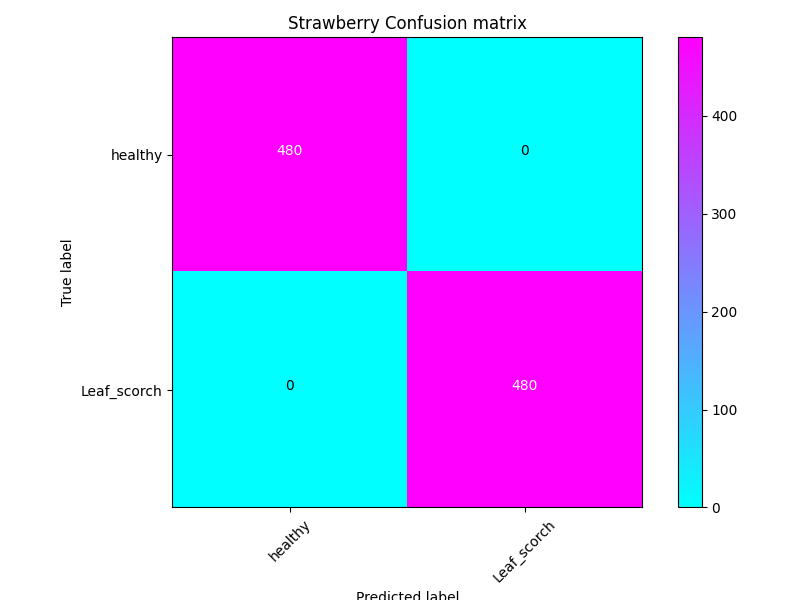
\includegraphics[width=11cm]{photos/chapter05/9.png}
      \caption{Strawberry Confusion Matrix.}
      \label{fig:strawberryConf}
    \end{figure}

  \item In the second model "Potato disease classification" obtained in 7200 images (80\% train and 20\% test).
    \begin{figure}[H]
      \centering
      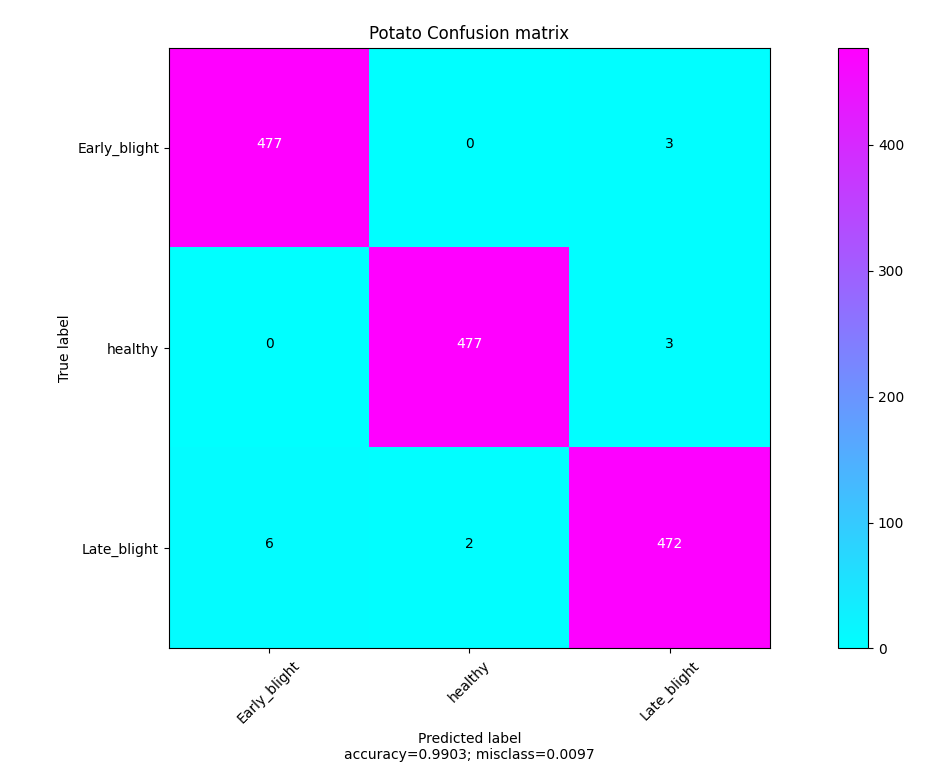
\includegraphics[width=11cm]{photos/chapter05/10.png}
      \caption{Potato Confusion Matrix.}
    \end{figure}

  \item In the third model "Pepper disease classification" obtained in 4800 images (80\% train and 20\% test).
    \begin{figure}[H]
      \centering
      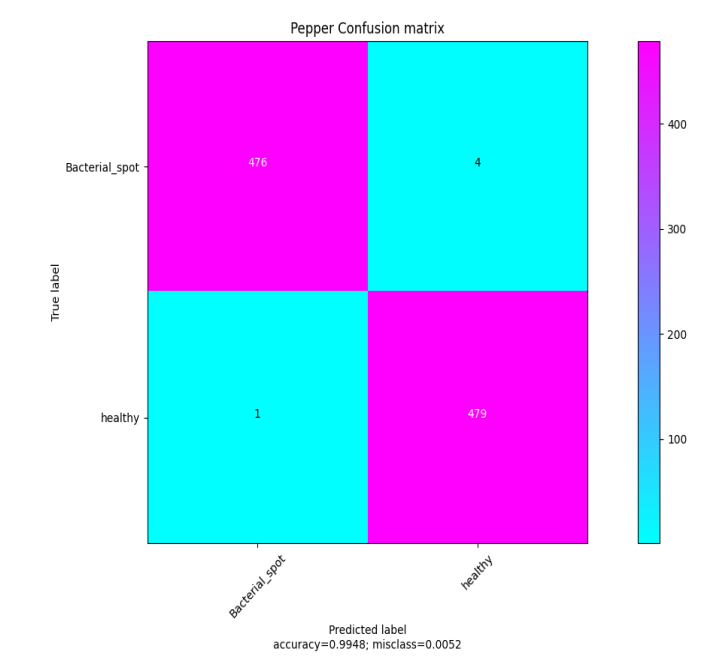
\includegraphics[width=10cm]{photos/chapter05/11.png}
      \caption{Pepper Confusion Matrix.}
    \end{figure}

  \item In the fourth model "Peach disease classification" obtained in 4800 images (80\% train and 20\% test).
    \begin{figure}[H]
      \centering
      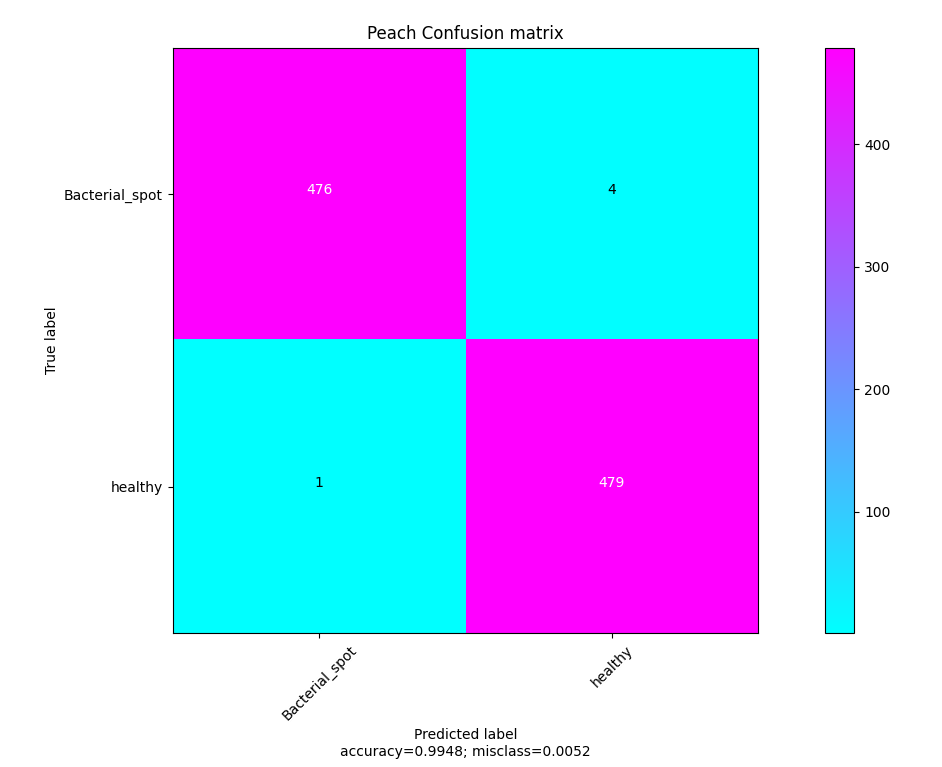
\includegraphics[width=10cm]{photos/chapter05/12.png}
      \caption{Peach Confusion Matrix.}
    \end{figure}

  \item In the fifth model "Grape disease classification" obtained in 9600 images (80\% train and 20\% test).
    \begin{figure}[H]
      \centering
      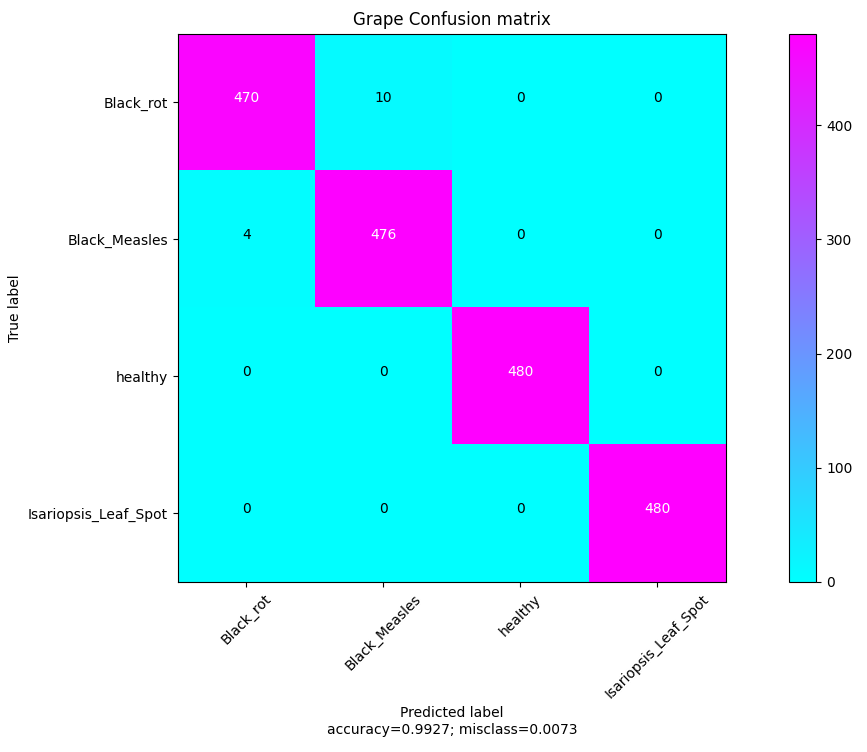
\includegraphics[width=10cm]{photos/chapter05/13.png}
      \caption{Grape Confusion Matrix.}
    \end{figure}

  \item In the sixth model "Cherry disease classification" obtained in 4800 images (80\% train and 20\% test).
    \begin{figure}[H]
      \centering
      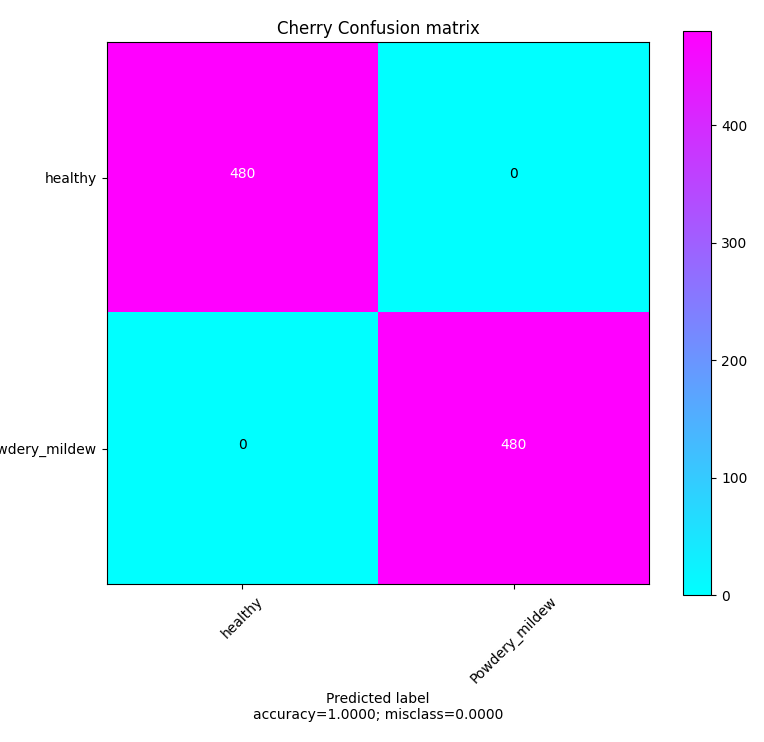
\includegraphics[width=9cm]{photos/chapter05/14.png}
      \caption{Charry Confusion Matrix.}
    \end{figure}

  \item In the seventh model "Apple disease classification" obtained in 7440 images (80\% train and 20\% test).
    \begin{figure}[H]
      \centering
      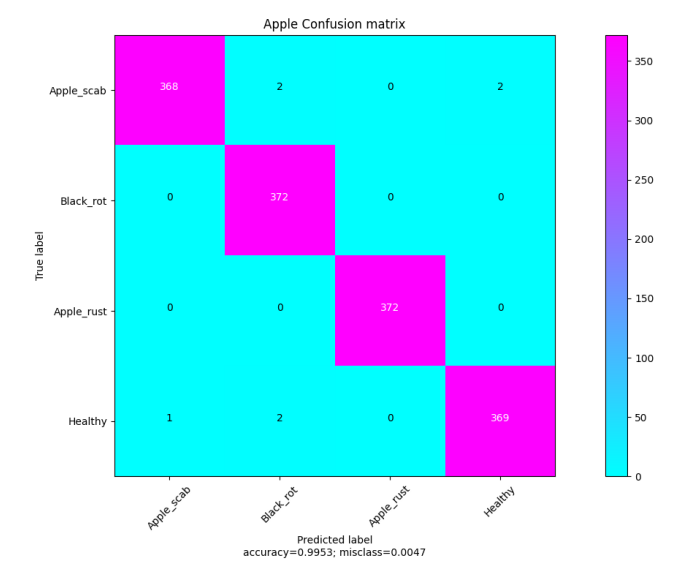
\includegraphics[width=10cm]{photos/chapter05/15.png}
      \caption{Apple Confusion Matrix.}
    \end{figure}

  \item In the eight model "Corn disease classification" obtained in 9600 images (80\% train and 20\% test).
    \begin{figure}[H]
      \centering
      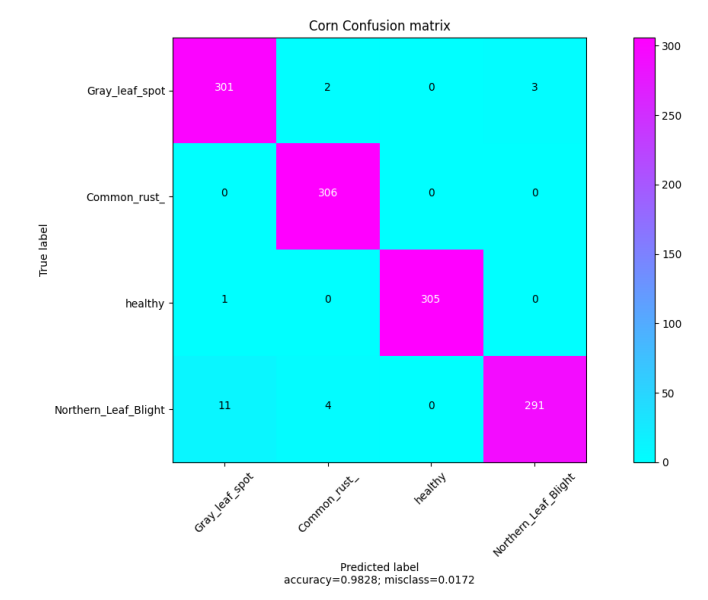
\includegraphics[width=10cm]{photos/chapter05/16.png}
      \caption{Corn Confusion Matrix.}
      \label{fig:cornConf}
    \end{figure}
\end{enumerate}

\noindent Figure (\ref{fig:exmaplePlantDis}) shows Examples of Plant Diseases.
\begin{figure}[H]
  \centering
  \begin{tabular}{ccc}
      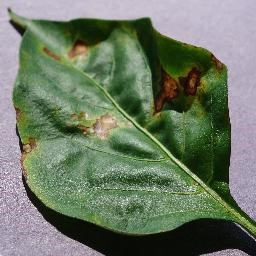
\includegraphics[width=3.3cm]{photos/chapter05/17.jpg} & 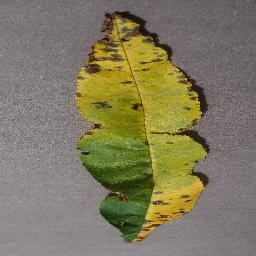
\includegraphics[width=3.3cm]{photos/chapter05/18.jpg} 
      & 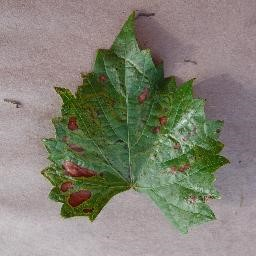
\includegraphics[width=3.3cm]{photos/chapter05/19.jpg} \\[3pt]
      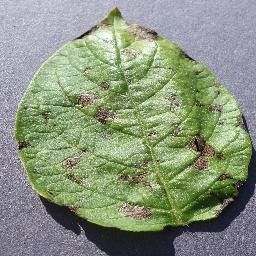
\includegraphics[width=3.3cm]{photos/chapter05/20.jpg} & 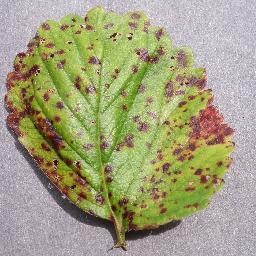
\includegraphics[width=3.3cm]{photos/chapter05/21.jpg} 
      & 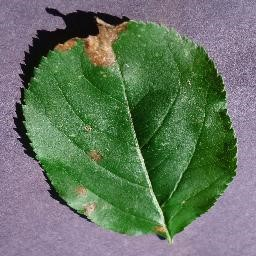
\includegraphics[width=3.3cm]{photos/chapter05/22.jpg} \\[3pt]
  \end{tabular}
  \caption{Examples of Plant Diseases.}
  \label{fig:exmaplePlantDis}
\end{figure}


\subsubsection{Scenario III: Ripeness assessment}

This scenario presents  ripeness assessment model using raw data. 
The results of object detection training using YOLOv5 on the real 
dataset that consist of 310 images of Strawberry  is discussed in 
this subsection. Table (\ref{tab:preform3}) shows the performance metrics Ripeness 
Assessment Model on this dataset of the third scenario.
Figure (\ref{fig:resultTrain}) shows Results of 'feature extraction' Training.

\begin{figure}[H]
  \centering
  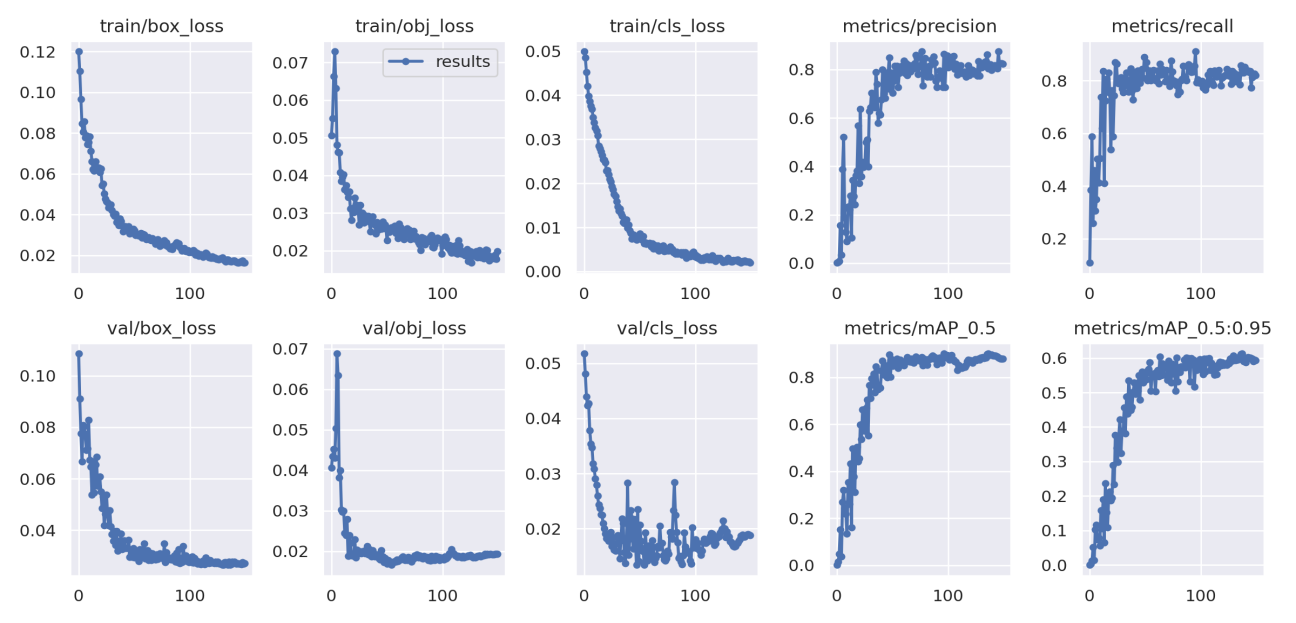
\includegraphics[width=\textwidth]{photos/chapter05/23.png}
  \caption{Results of 'feature extraction' Training.}
  \label{fig:resultTrain}
\end{figure}

\begin{table}[H]
  \setlength\arrayrulewidth{0.5pt}
  \renewcommand{\arraystretch}{1.5}
  \begin{tabularx}{\textwidth}{|p{3.4cm}|X|X|X|X|}
      \hline
      \multicolumn{5}{|c|}{\textbf{Real Dataset of Strawberry}} \\ \hline
      \textbf{Model} & \textbf{Class} & \textbf{Recall} & \textbf{Precision} & \textbf{mAP\@.5} \\ \hline
      & all & 0.902 & 0.855 & 0.912 \\ \cline{2-5}
      & green & 0.915 & 0.841 & 0.905 \\ \cline{2-5}
      & pink & 0.875 & 0.951 & 0.955 \\ \cline{2-5}
      & red & 0.933 & 0.767 & 0.876 \\ \cline{2-5}
      \multirow{-5}{*}{\textbf{YOLO-V5}} & white & 0.886 & 0.861 & 0.914 \\ \hline
  \end{tabularx}
  \caption{Performance metrics for dataset of Ripeness assessment model.}
  \label{tab:preform3}
\end{table}

Table (\ref{tab:preform3}) shows the performance of YOLOv5 of Object Detection model for 
classification considering Real dataset of  Strawberry . For YOLOv5 with real dataset of 
Strawberry, it is noticed that the obtained accuracy is 87.8\%, the obtained recall percentage 
is 90.2\%, where the percentage of correctly recognized plant images against the total number 
of actual plant images and the precision 85.5\%.
Figure (\ref{fig:ripConf}) shows Ripeness Confusion Matrix.

\begin{figure}[H]
  \centering
  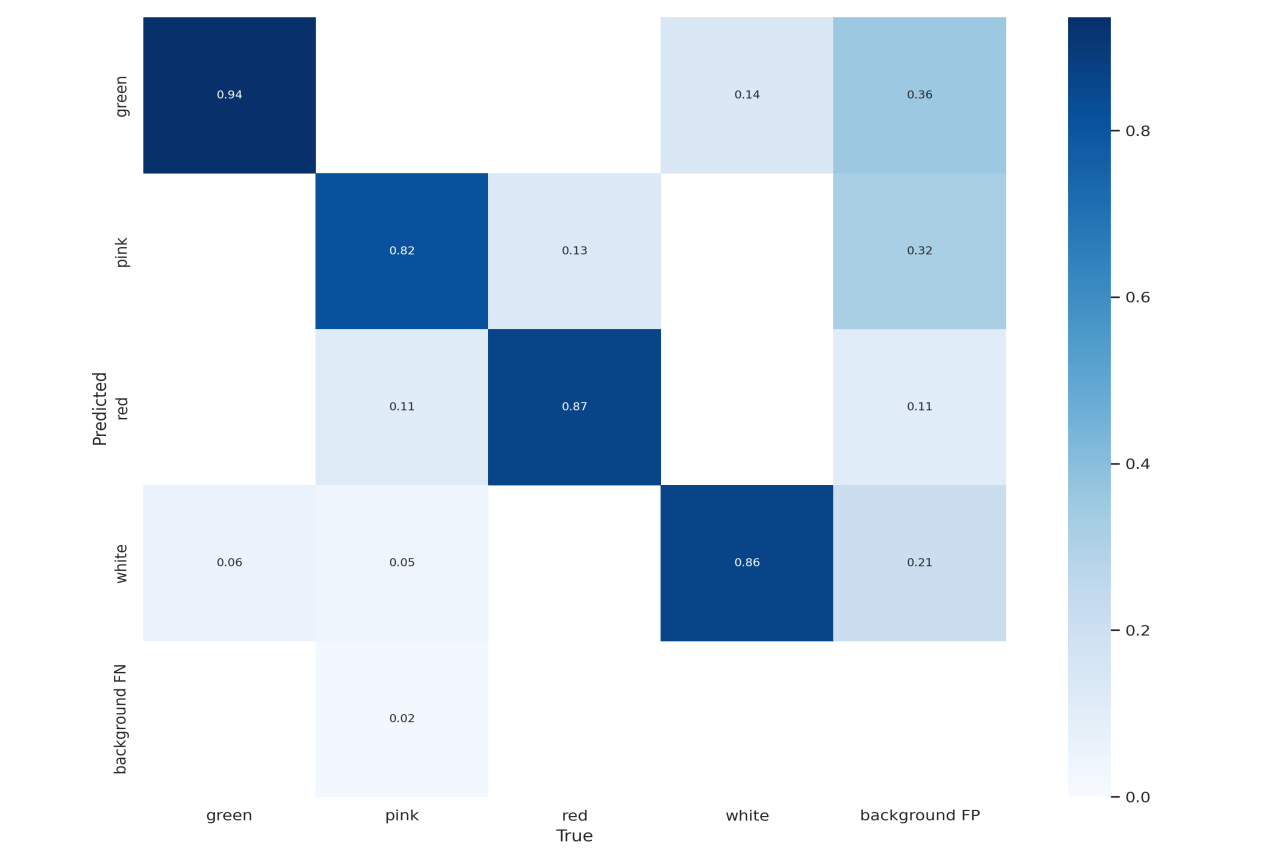
\includegraphics[width=12cm]{photos/chapter05/24.png}
  \caption{Ripeness Confusion Matrix.}
  \label{fig:ripConf}
\end{figure}

\begin{figure}[H]
  \centering
  \begin{tabular}{cc}
      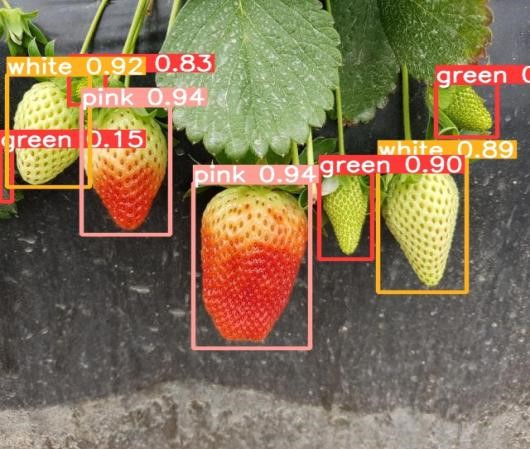
\includegraphics[width=0.4\textwidth]{photos/chapter05/25.jpg} & 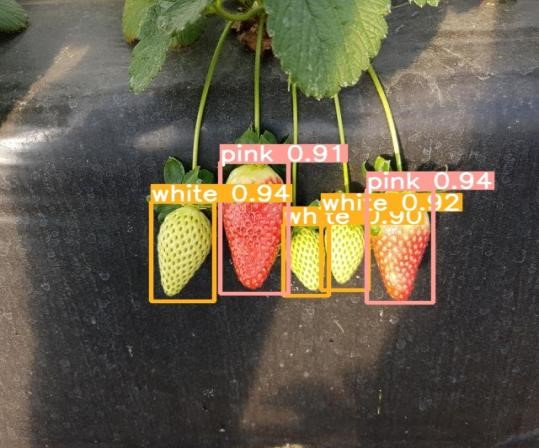
\includegraphics[width=0.4\textwidth]{photos/chapter05/26.jpg} \\[2pt]
      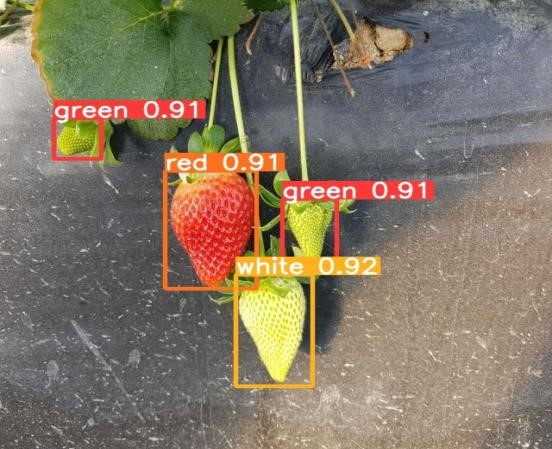
\includegraphics[width=0.4\textwidth]{photos/chapter05/28.jpg} & 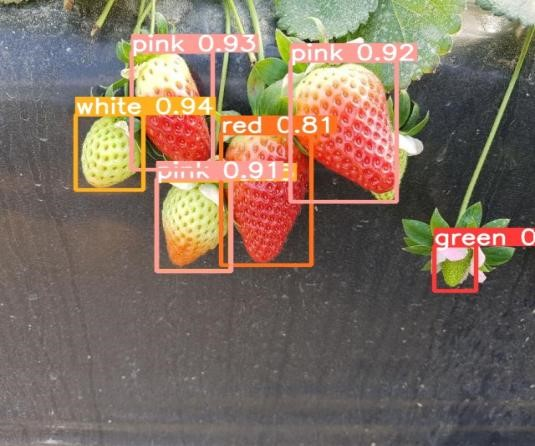
\includegraphics[width=0.4\textwidth]{photos/chapter05/27.jpg} \\[2pt]
  \end{tabular}
  \caption{Examples of Object Detection.}
\end{figure}
